\chapter{Einleitung}
Durch den stetigen Fortschritt und der steigenden Komplexität der Anwendungen,
werden immer größere Datenmengen erzeugt. Sei es im privaten Umfeld durch die
Benutzung von Social-Media Platformen wie Facebook, Twitter,~\dots oder im gewerblichen
Umfeld durch medinische Daten, Börsendaten,~\dots . Durch die stetige Vernetzung
von Alltagsgegenständen, welches man unter dem Begriff IoT\footnote{Internet of the Things}
zusammenfassen kann, stiegen diese Datenmengen nochmals sehr stark an. Dies hat
zur Folge, dass die Verarbeitung dieser Datenmengen immer komplexer wird und dies
mit nur einem einzelnen Rechner nicht mehr möglich ist. Dies wird als \gls{BigData}
bezeichnet. Bei der Verarbeitung von großen Datenmengen wird zwischen zwei
unterschiedlichen Methoden unterschieden Batch-Processing und Stream-Processing.
Beim Batch-Processing wird eine feste Datenmenge in kleinere Einheiten unterteilt.
Diese Teildaten werden dann von mehreren Rechnern einzeln bearbeitet und
anschließen die Ergebnisse wieder kombiniert. Beim Stream-Processing gibt es
keine feste Menge, sondern die Daten kommen kontinuierlich in die Verarbeitung.
Dadurch ist es möglich die Daten in Echtzeit zu verarbeiten. Stream-Processing
eignet sich für folgende Einsatzgebiete:

\begin{itemize}
\item Fehlererkennung zum Beispiel bei Kreditkarten
\item Spracherkennung
\item Log-Analysen
\item Event-Verarbeitung
\end{itemizze}

\begin{figure}
\centering
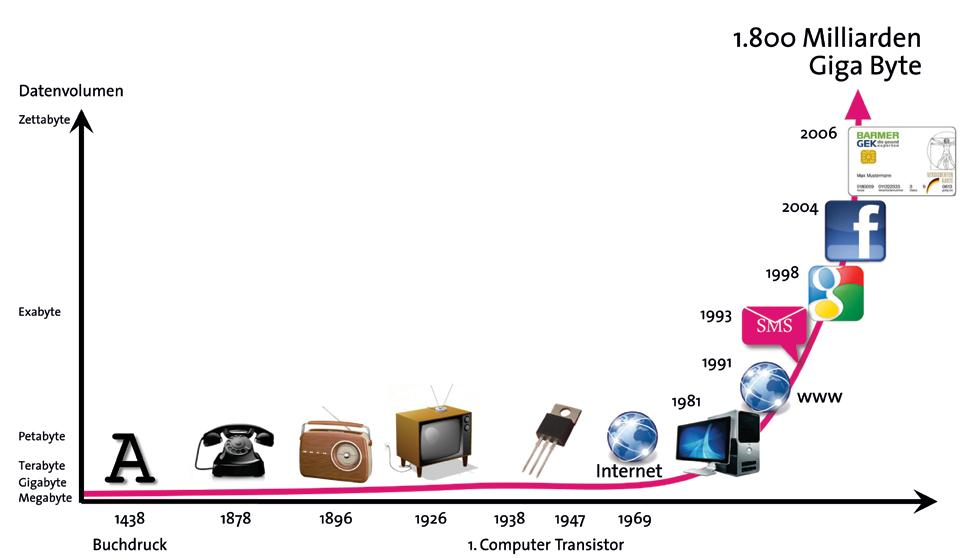
\includegraphics[scale=0.375]{../material/images/bitkom-lf-bigdata-2012-data_grow.jpg}
\caption{Erhöhung der Datenmenge von 1400 bis 2006 \parencite{Weber2012}}
\label{fig:data-grow}
\end{figure}

Die Daten können dabei je nach Anwendungsfall unterschiedlich strukturiert sein.
Es wird dabei unterschieden zwischen unstrukturierten, semi-strukturieren
und strukturierten Daten. Strukturierte Daten haben eine feste Struktur. Bei
semi-strukturieren Daten sind lediglich einzelne Bausteine definiert,
jedoch nicht wie die Daten aus den Bausteinen entstehen. Bei unstrukturierten
Daten gibt es überhaupt keine Struktur, sondern lediglich die Information, um
welche Art von Daten es sich handelt.

In der heutigen Welt spielen vor allem Graphen eine wichtige Rolle. Da 
Unternehmen heute die Daten aus verschiedenen Quellen kombinieren wollen, um zum
Beispiel zusätzliche Werbung zu schalten. Als Beispiel jemand kauft ein Paar
Schuhe und bekommt dazu ein Angebot zu einer Tasche angezeigt, weil zum
Beispiel anderen Kunden beide Artikel gekauft haben. Ein anderes Beispiel von
Facebook ist die Liste der Personen, welche der Benutzer eventuell kennt.
Dabei werden die Informationen des Benutzers mit den Informationen der Freunde
bzw. deren Freunde kombiniert. Existiert nun eine Person, welche zum Beispiel
in dieselbe Schule gegangen ist und nur Freund eines Freundes ist, wird diese
Person der Liste der Personen hinzugefügt, welche der Benutzer eventuell kennt.

\section{Motivation}
Wenn beide Welten \gls{BigData} hier Stream-Processing und Graphen miteinander
kombiniert werden, ergeben sich die verschiedene Problemsituationen, welche
gelöst werden müssen. Zunächst einmal sind Graphen komplexe Datenstrukturen,
diese müssen in geeigneter Weise in den Programmen bzw. im Speicher geeignet
abgebildet werden können um eine Verarbeitung zu ermöglichen. Des Weiteren ist
es nicht immer möglich und notwendig den gesamten Graphen zu speichern, sondern
es steht nur ein Teilgraph zur Verfügung.

\section{Ziel der Arbeit}
Ziel der Arbeit ist es die gewählten Bibliotheken hinsichtlich geeigneter
Kriterien zu vergleichen und diese anhand eines Beispieles praktisch zu
demonstrieren.

Dabei sollen die auftretenden Probleme bzw. Grenzen erläutert und mögliche
Lösungen bzw. Erweiterungspunkte der Bibliotheken vorgestellt werden.

\section{Aufbau der Arbeit}
Im nächsten Kapitel werden die verwendeten Technologien und Softwaresysteme
beschrieben, um einen Überblick zu bekommen. Dann wird das Design des Beispieles
für die jeweilige Bibliothek erläutert und die sich schon abzeichnenden Probleme
werden beschrieben. Danach wird das Design anhand der technischen Umsetzung
dargelegt und die auftretenden Probleme beschrieben. Abschließend folgt eine
Zusammenfassung und ein Ausblick auf zukünftige Schritte.
